\documentclass[draft]{agujournal2019}
\usepackage{url}
\usepackage{lineno}
\usepackage[inline]{trackchanges}
\usepackage{soul}
\linenumbers

\draftfalse

\journalname{JGR: Solid Earth}

\begin{document}

\title{Supplement to: Depth and thickness of tectonic tremor in the northeastern Olympic Peninsula}

\authors{A. Ducellier\affil{1}, K. C. Creager\affil{1}}

\affiliation{1}{University of Washington}

\correspondingauthor{Ariane Ducellier}{ducela@uw.edu}

\newpage

\begin{figure}
\noindent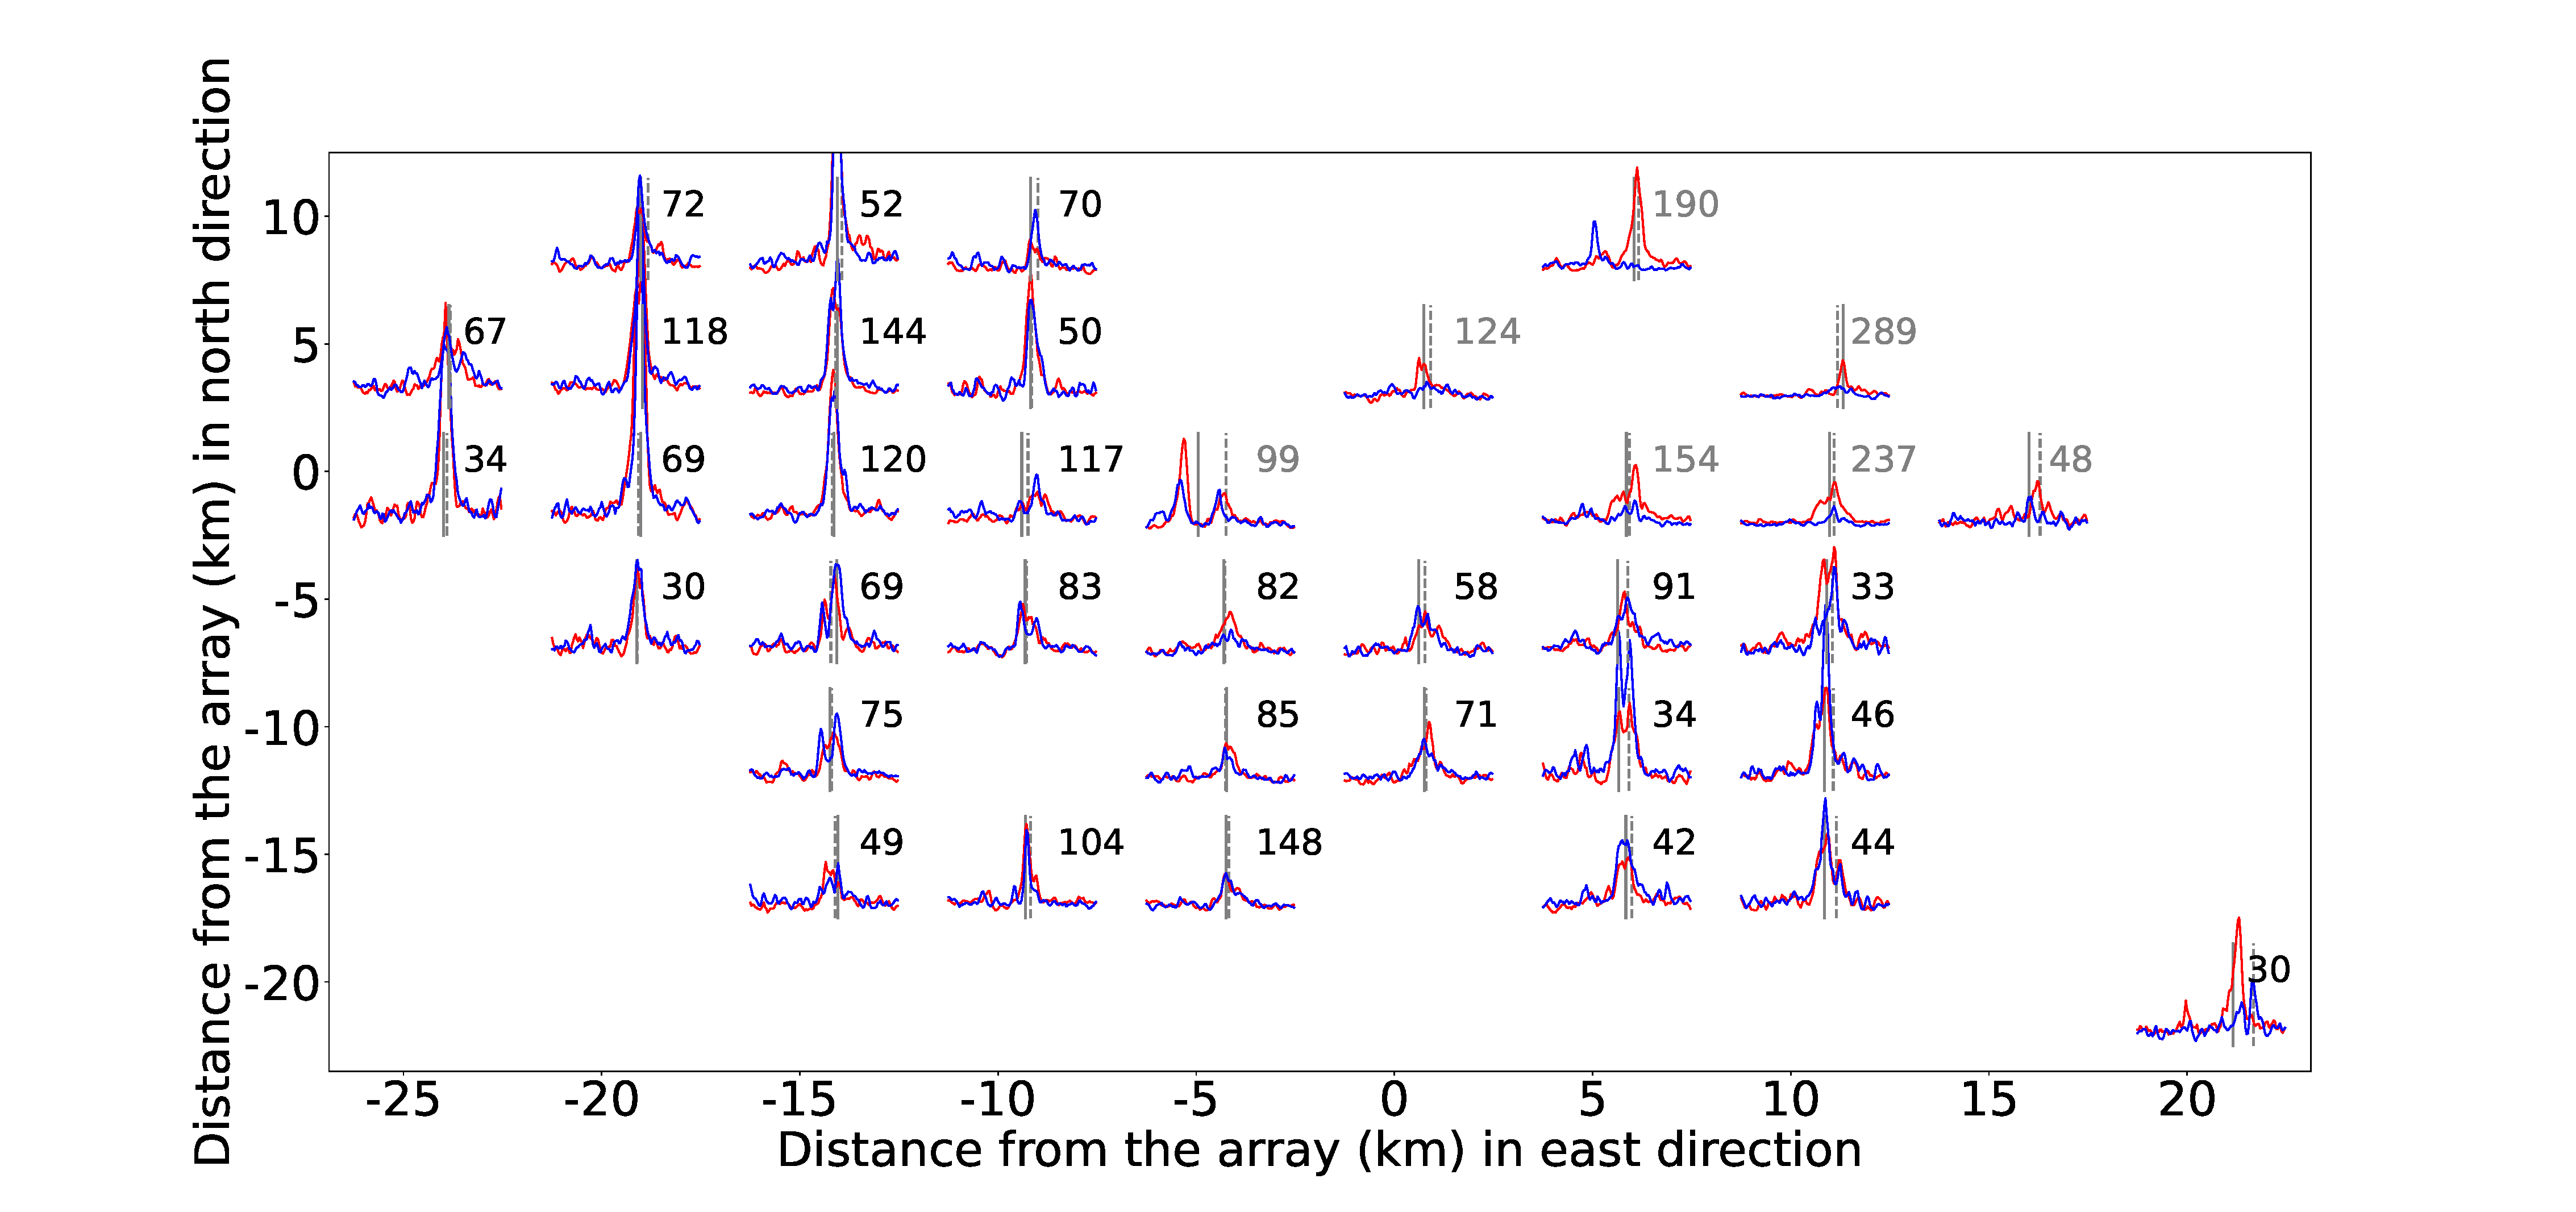
\includegraphics[width=\textwidth, trim={5cm 0.5cm 7.5cm 1.5cm},clip]{figures/BH_PWS_PWS_0.eps}
\caption{Stacks of the envelopes of the cross correlation signals for different positions of the tremor source relative to the Burnt Hill array. See caption of Figure 4 for an explanation of this figure.}
\label{pngfiguresample}
\end{figure}

\begin{figure}
\noindent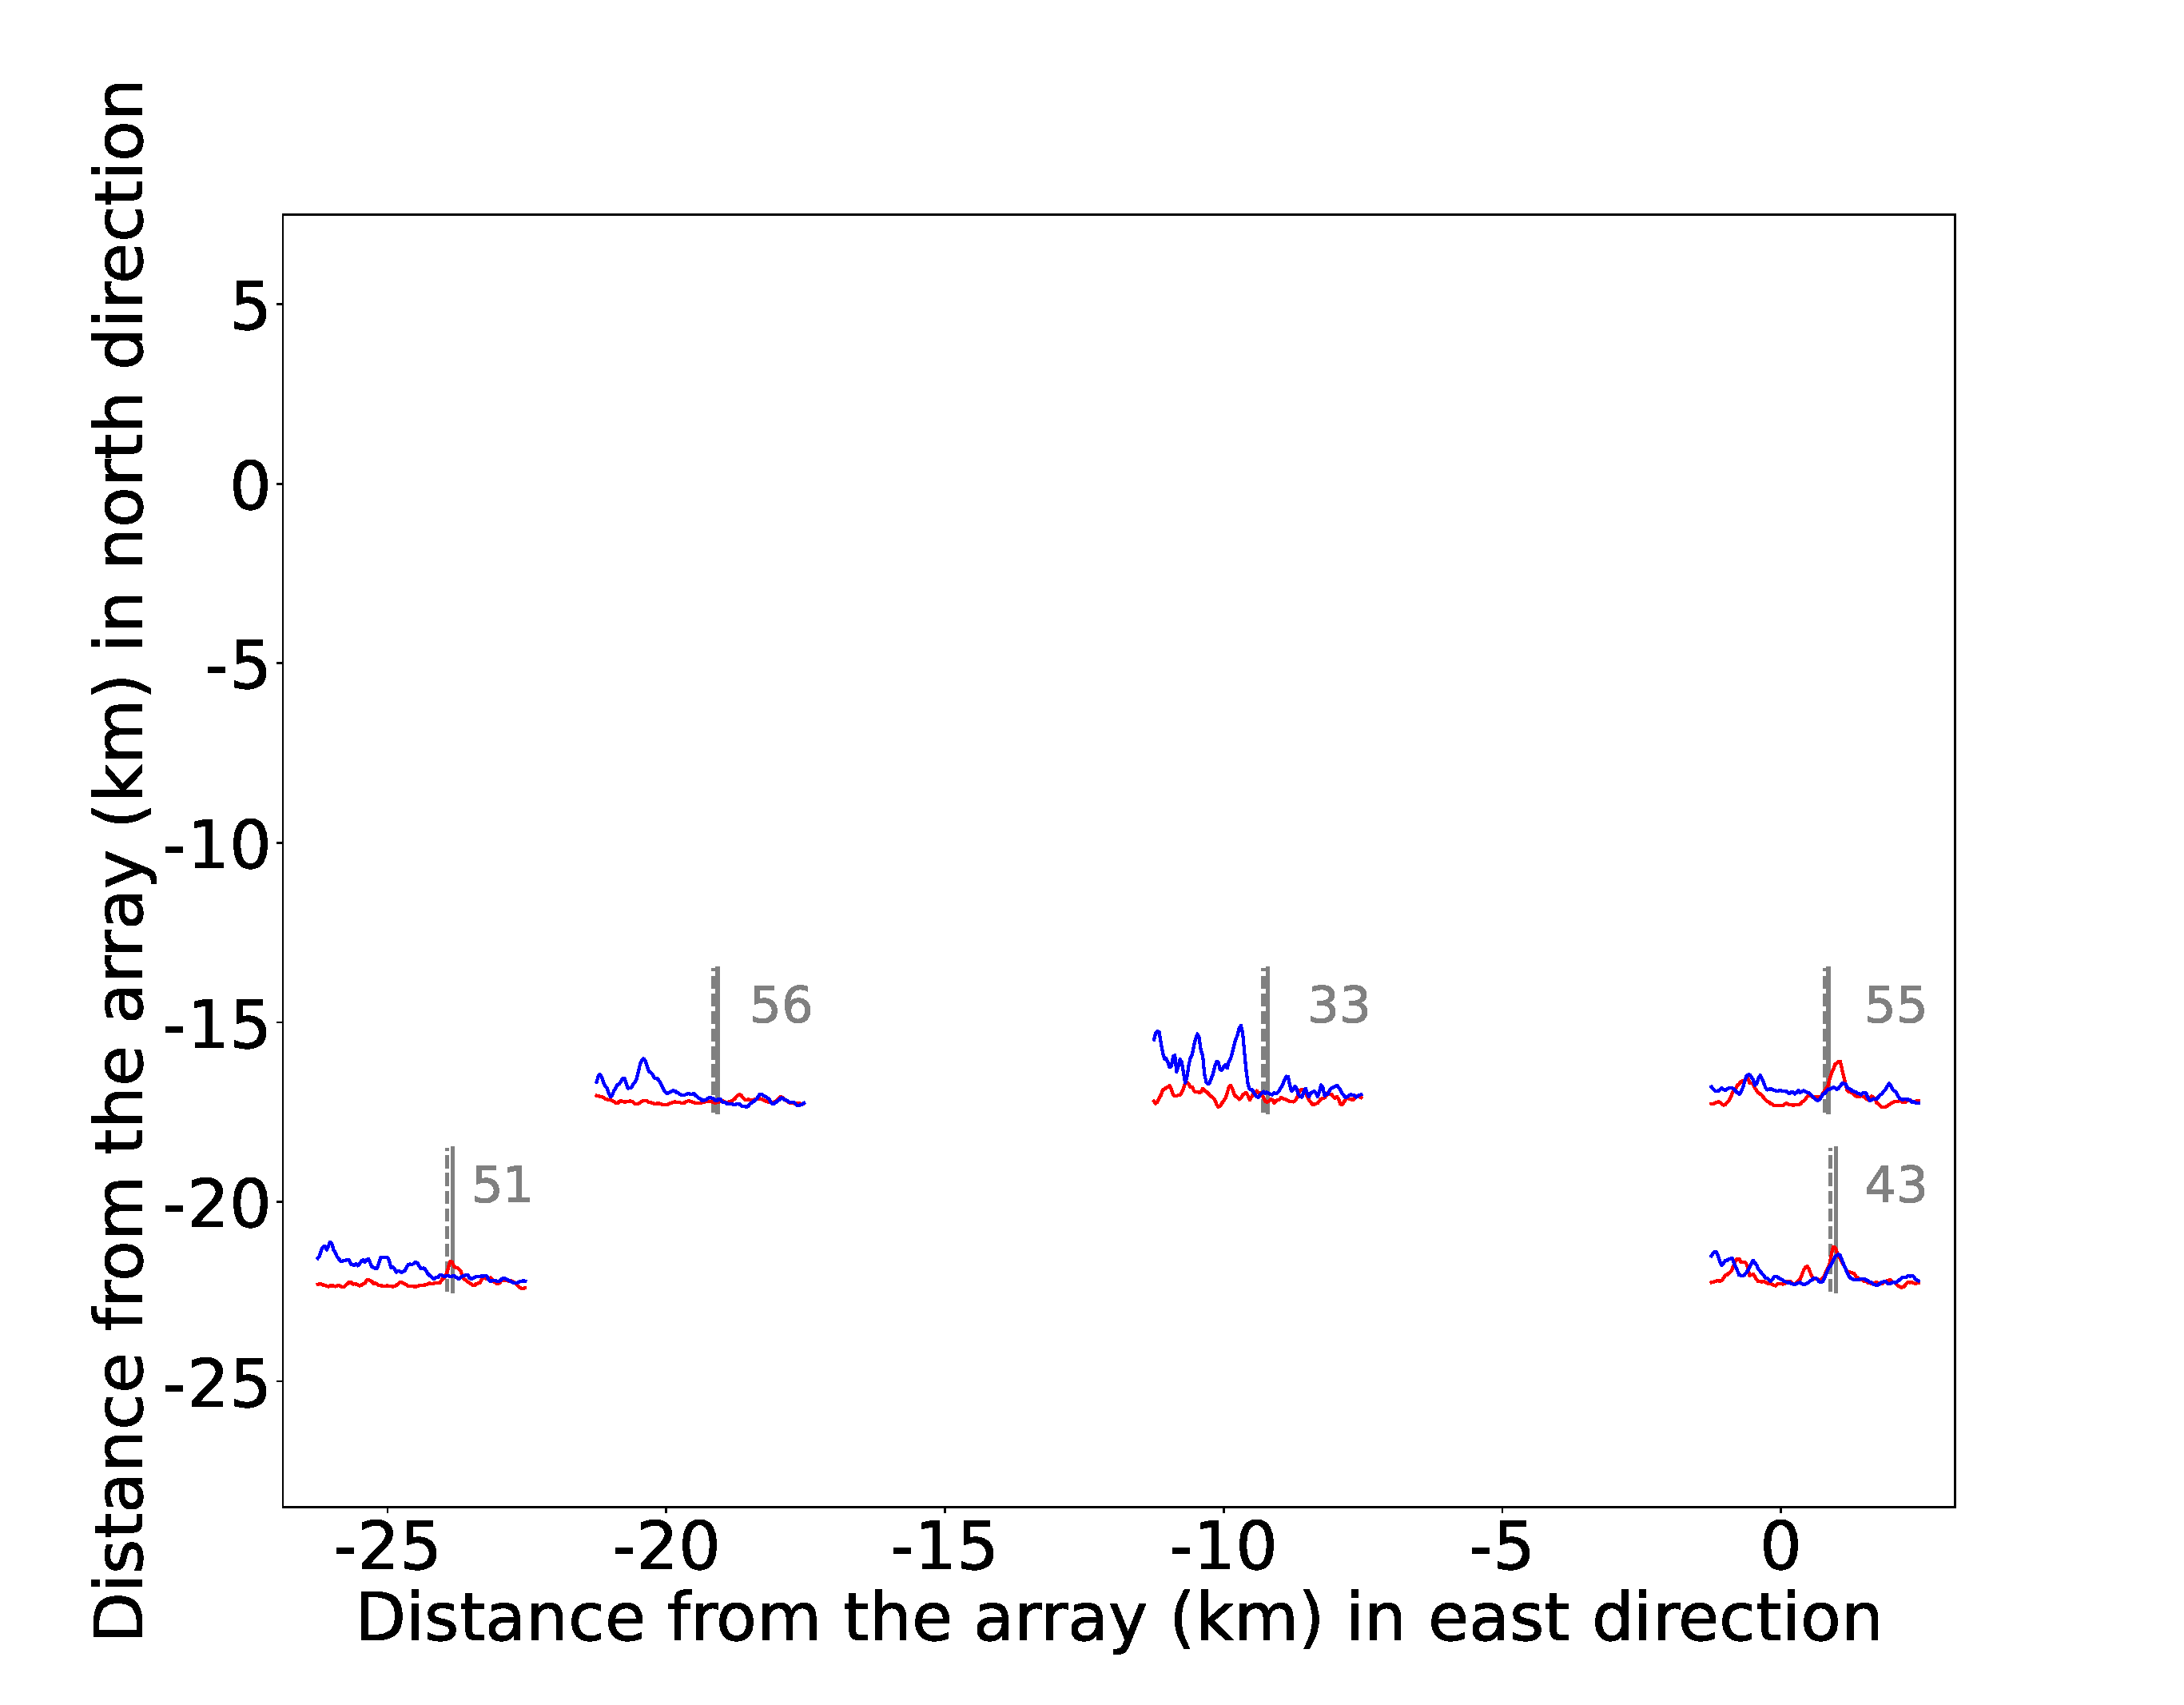
\includegraphics[width=\textwidth, trim={1.5cm 1cm 4.5cm 1.5cm},clip]{figures/CL_PWS_PWS_0.eps}
\caption{Stacks of the envelopes of the cross correlation signals for different positions of the tremor source relative to the Cat Lake array. See caption of Figure 4 for an explanation of this figure.}
\label{pngfiguresample}
\end{figure}

\begin{figure}
\noindent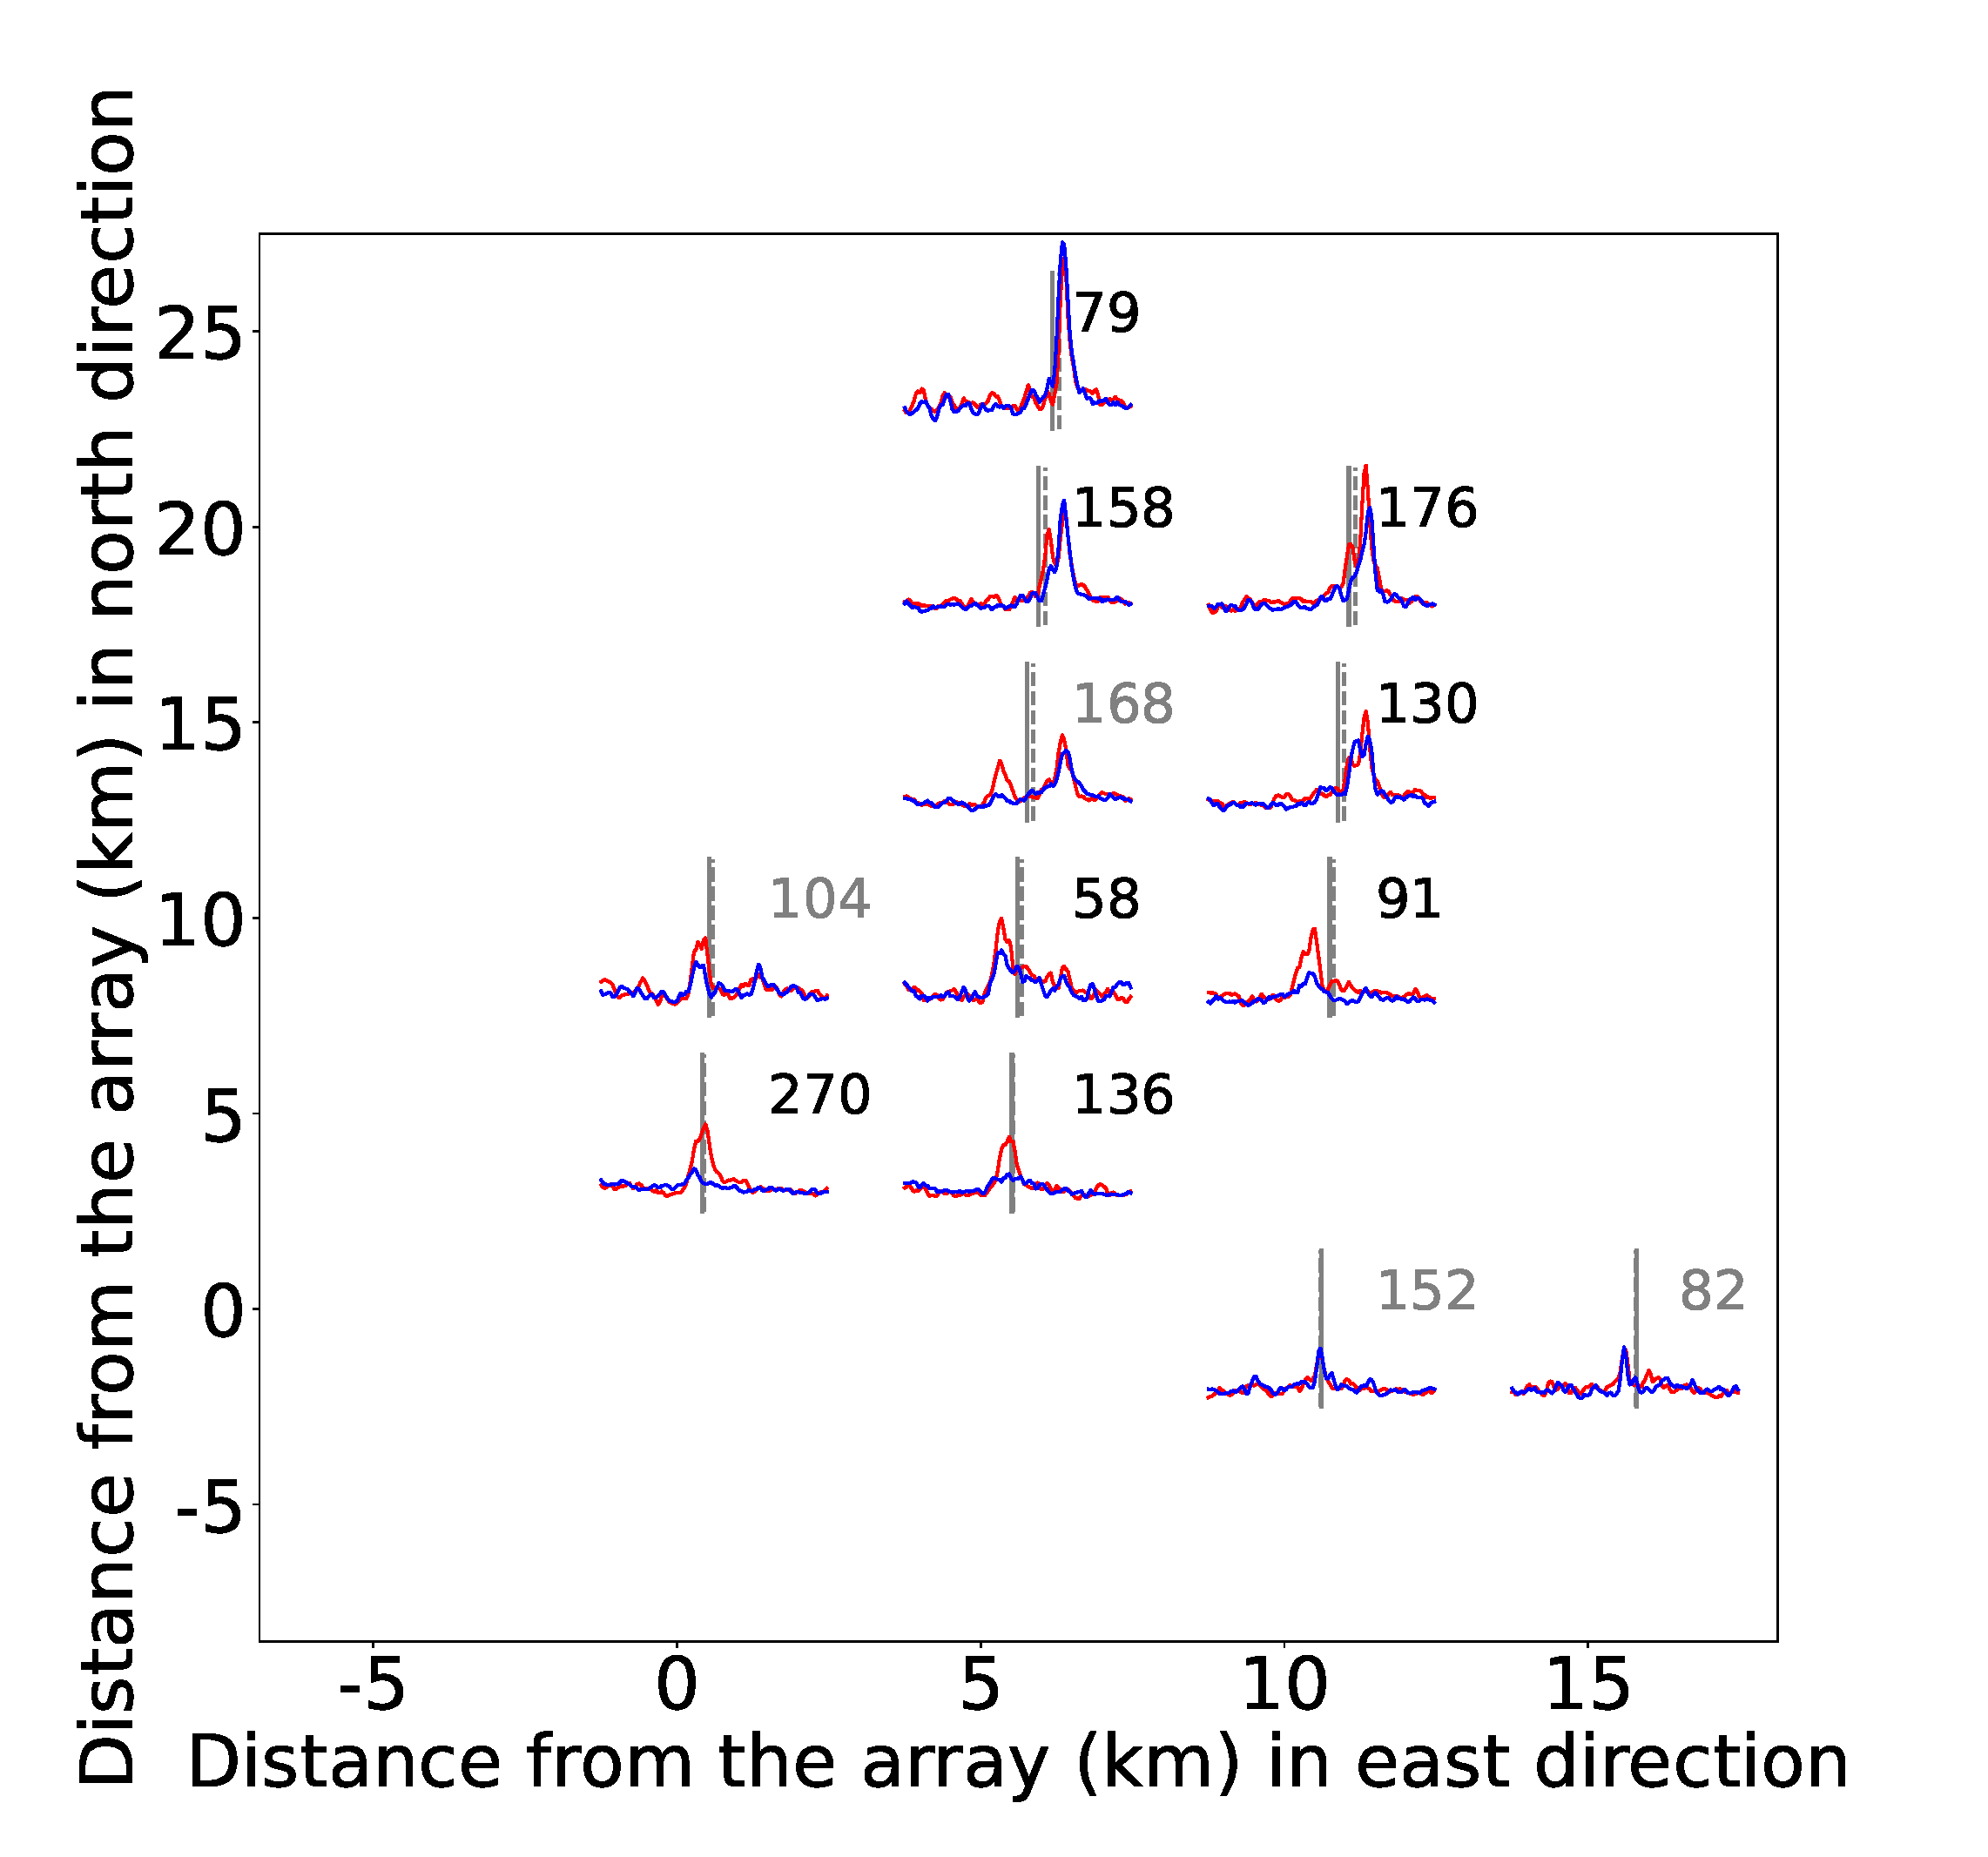
\includegraphics[width=\textwidth, trim={1cm 0.5cm 2.5cm 1.5cm},clip]{figures/DR_PWS_PWS_0.eps}
\caption{Stacks of the envelopes of the cross correlation signals for different positions of the tremor source relative to the Danz Ranch array. See caption of Figure 4 for an explanation of this figure.}
\label{pngfiguresample}
\end{figure}

\begin{figure}
\noindent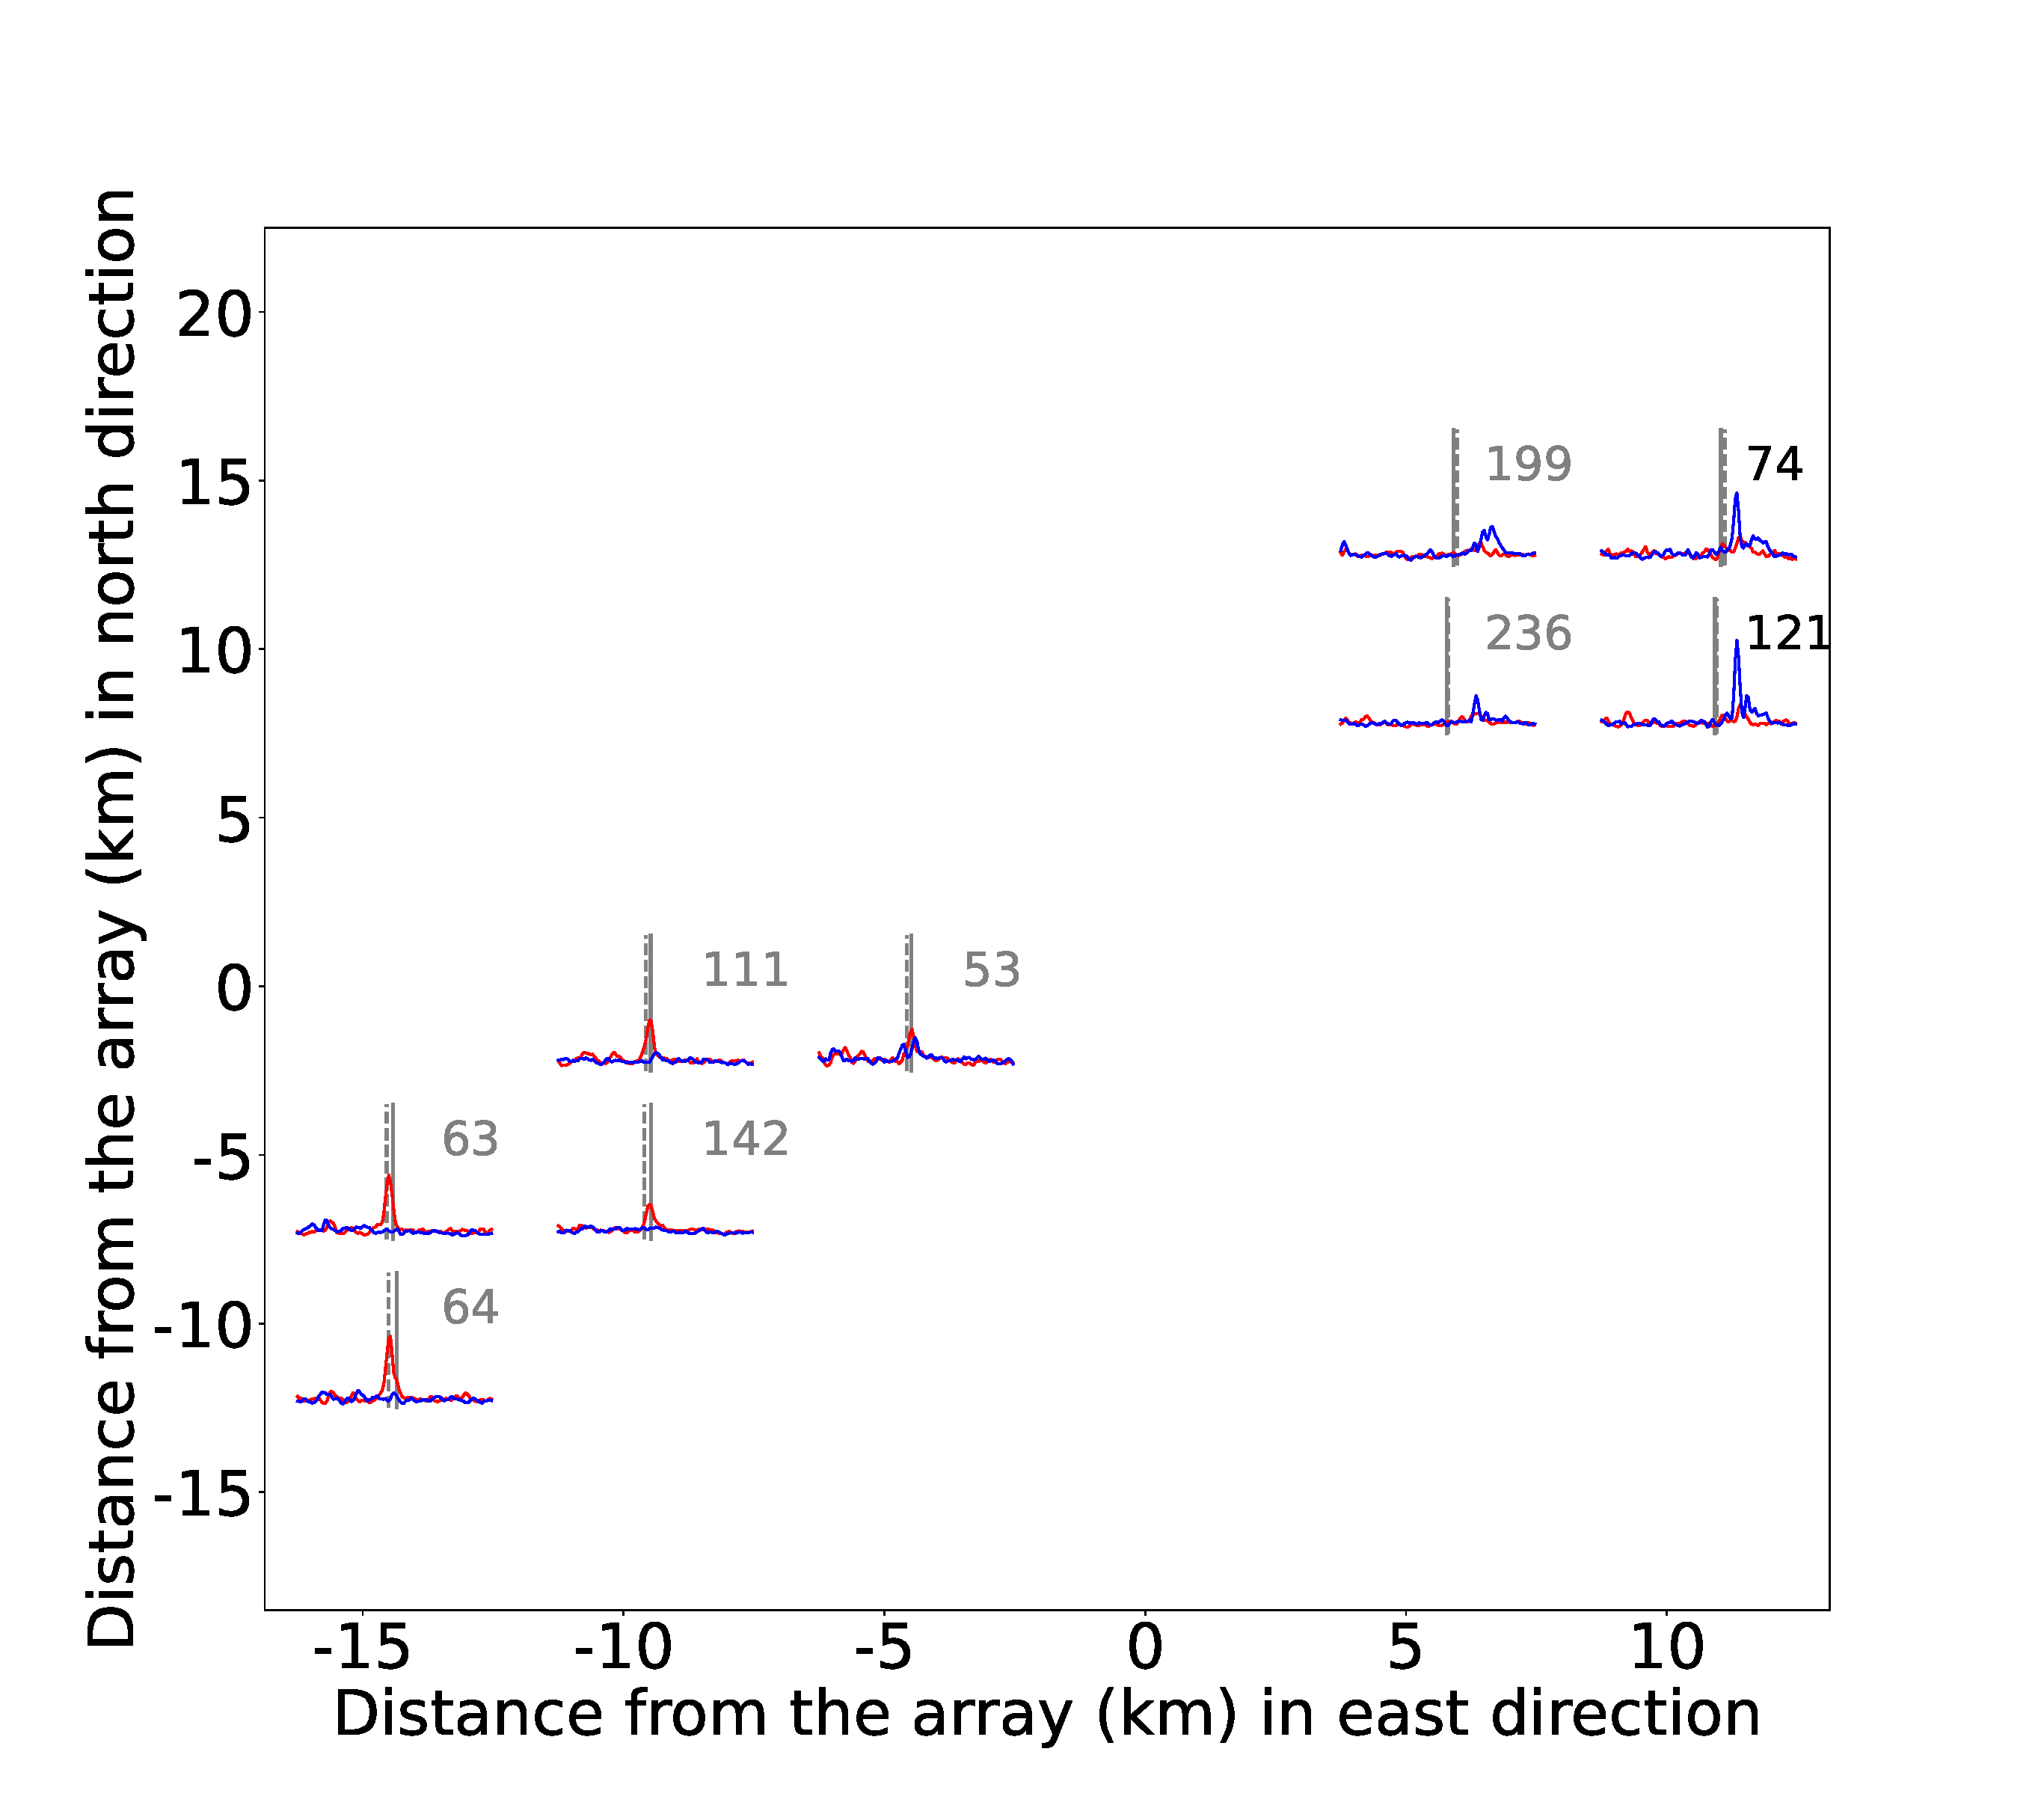
\includegraphics[width=\textwidth, trim={1.5cm 1cm 4.5cm 4cm},clip]{figures/GC_PWS_PWS_0.eps}
\caption{Stacks of the envelopes of the cross correlation signals for different positions of the tremor source relative to the Gold Creek array. See caption of Figure 4 for an explanation of this figure.}
\label{pngfiguresample}
\end{figure}

\begin{figure}
\noindent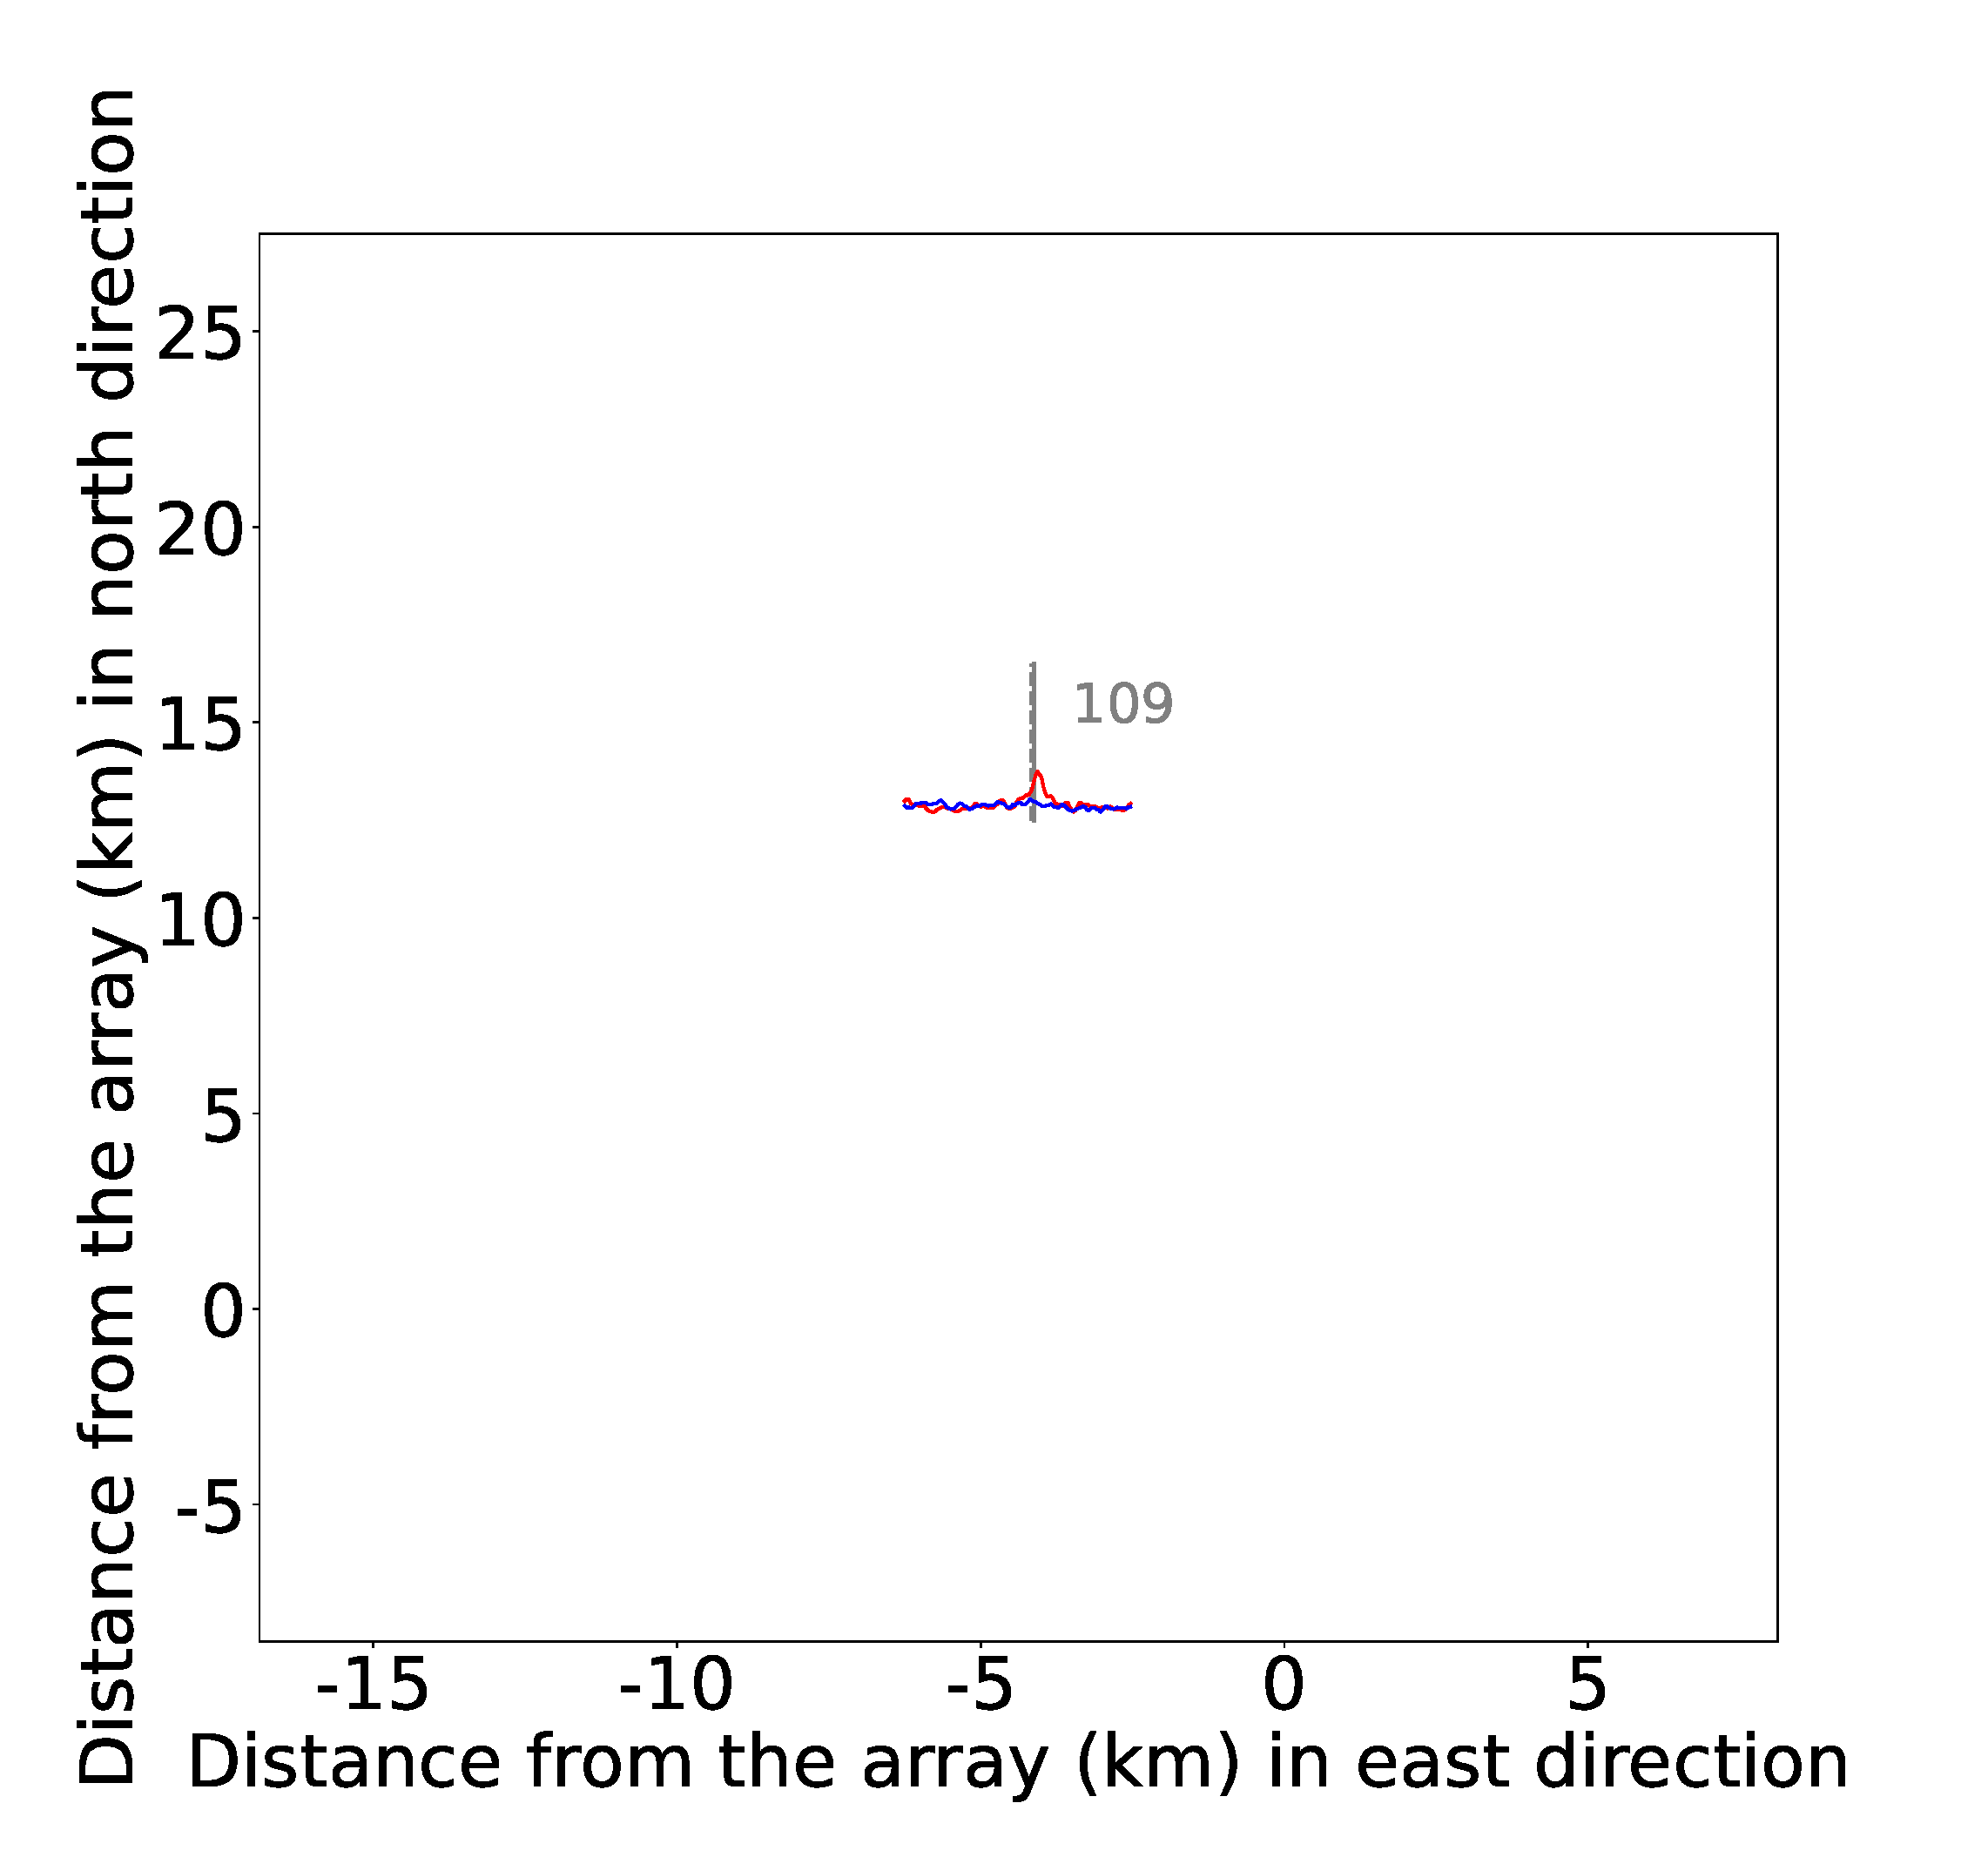
\includegraphics[width=\textwidth, trim={1cm 0.5cm 2.5cm 1.5cm},clip]{figures/LC_PWS_PWS_0.eps}
\caption{Stacks of the envelopes of the cross correlation signals for different positions of the tremor source relative to the Lost Cause array. See caption of Figure 4 for an explanation of this figure.}
\label{pngfiguresample}
\end{figure}

\begin{figure}
\noindent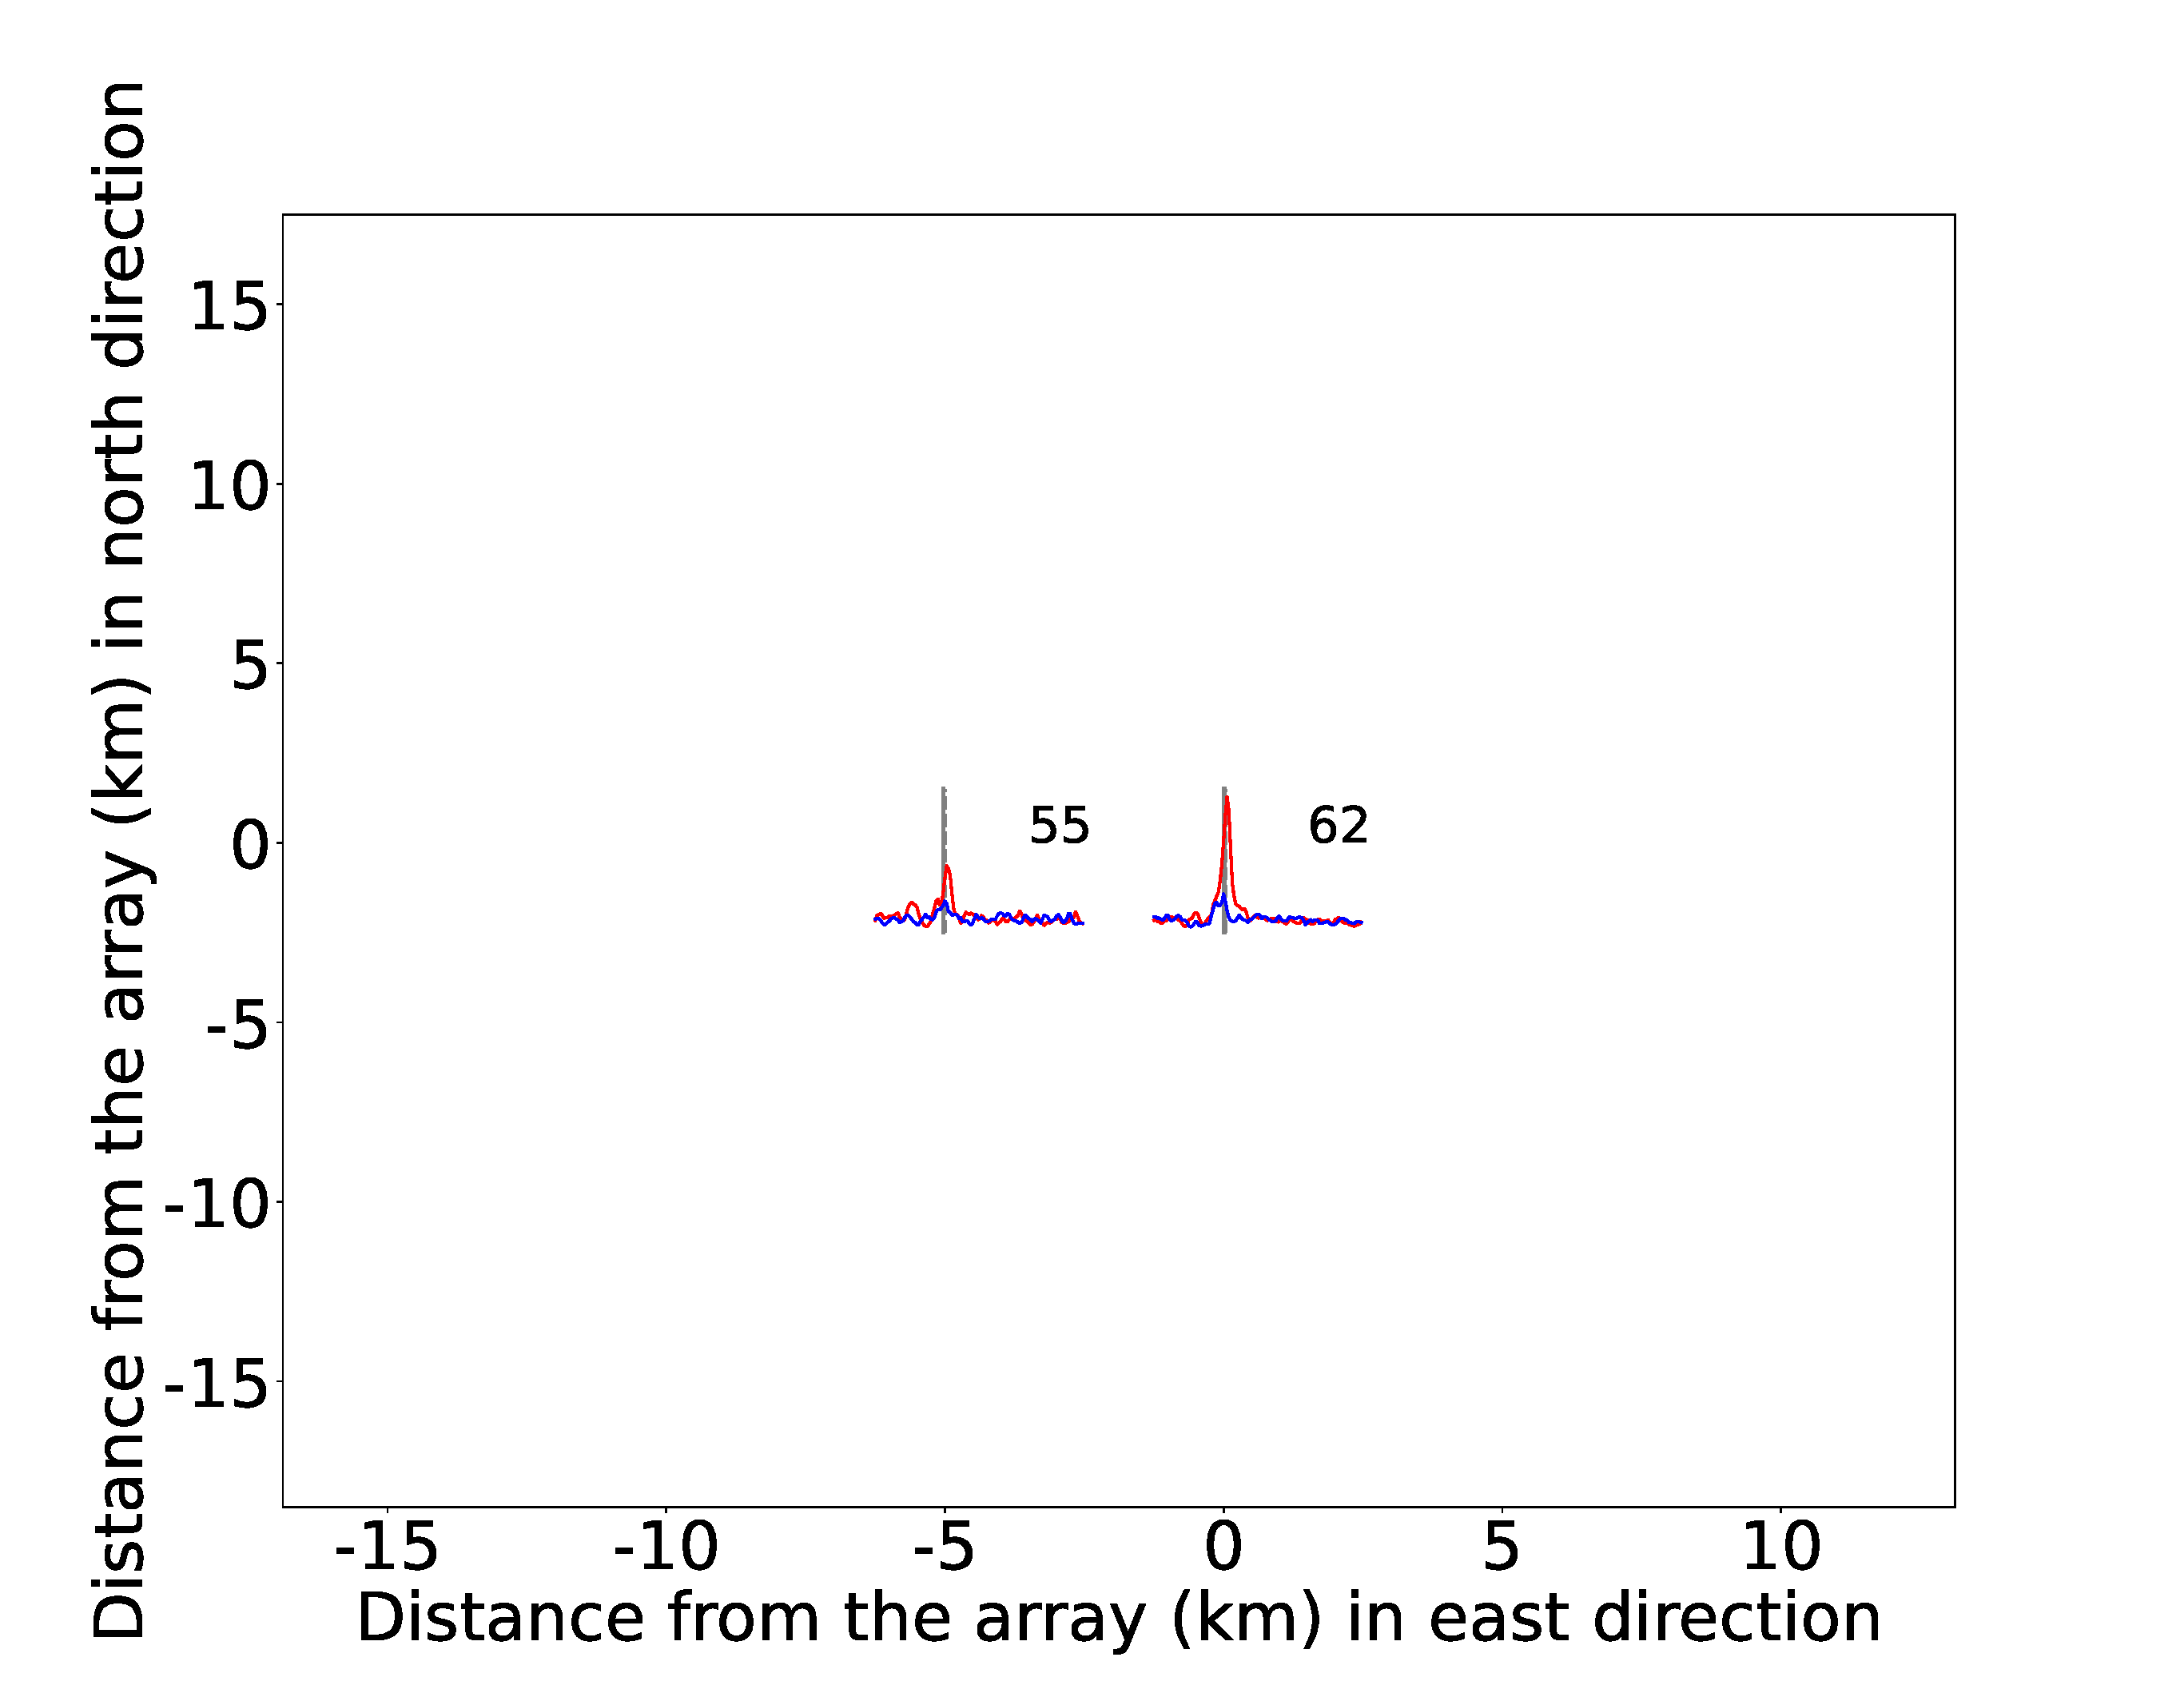
\includegraphics[width=\textwidth, trim={1.5cm 0.5cm 4.5cm 1.5cm},clip]{figures/PA_PWS_PWS_0.eps}
\caption{Stacks of the envelopes of the cross correlation signals for different positions of the tremor source relative to the Port Angeles array. See caption of Figure 4 for an explanation of this figure.}
\label{pngfiguresample}
\end{figure}

\begin{figure}
\noindent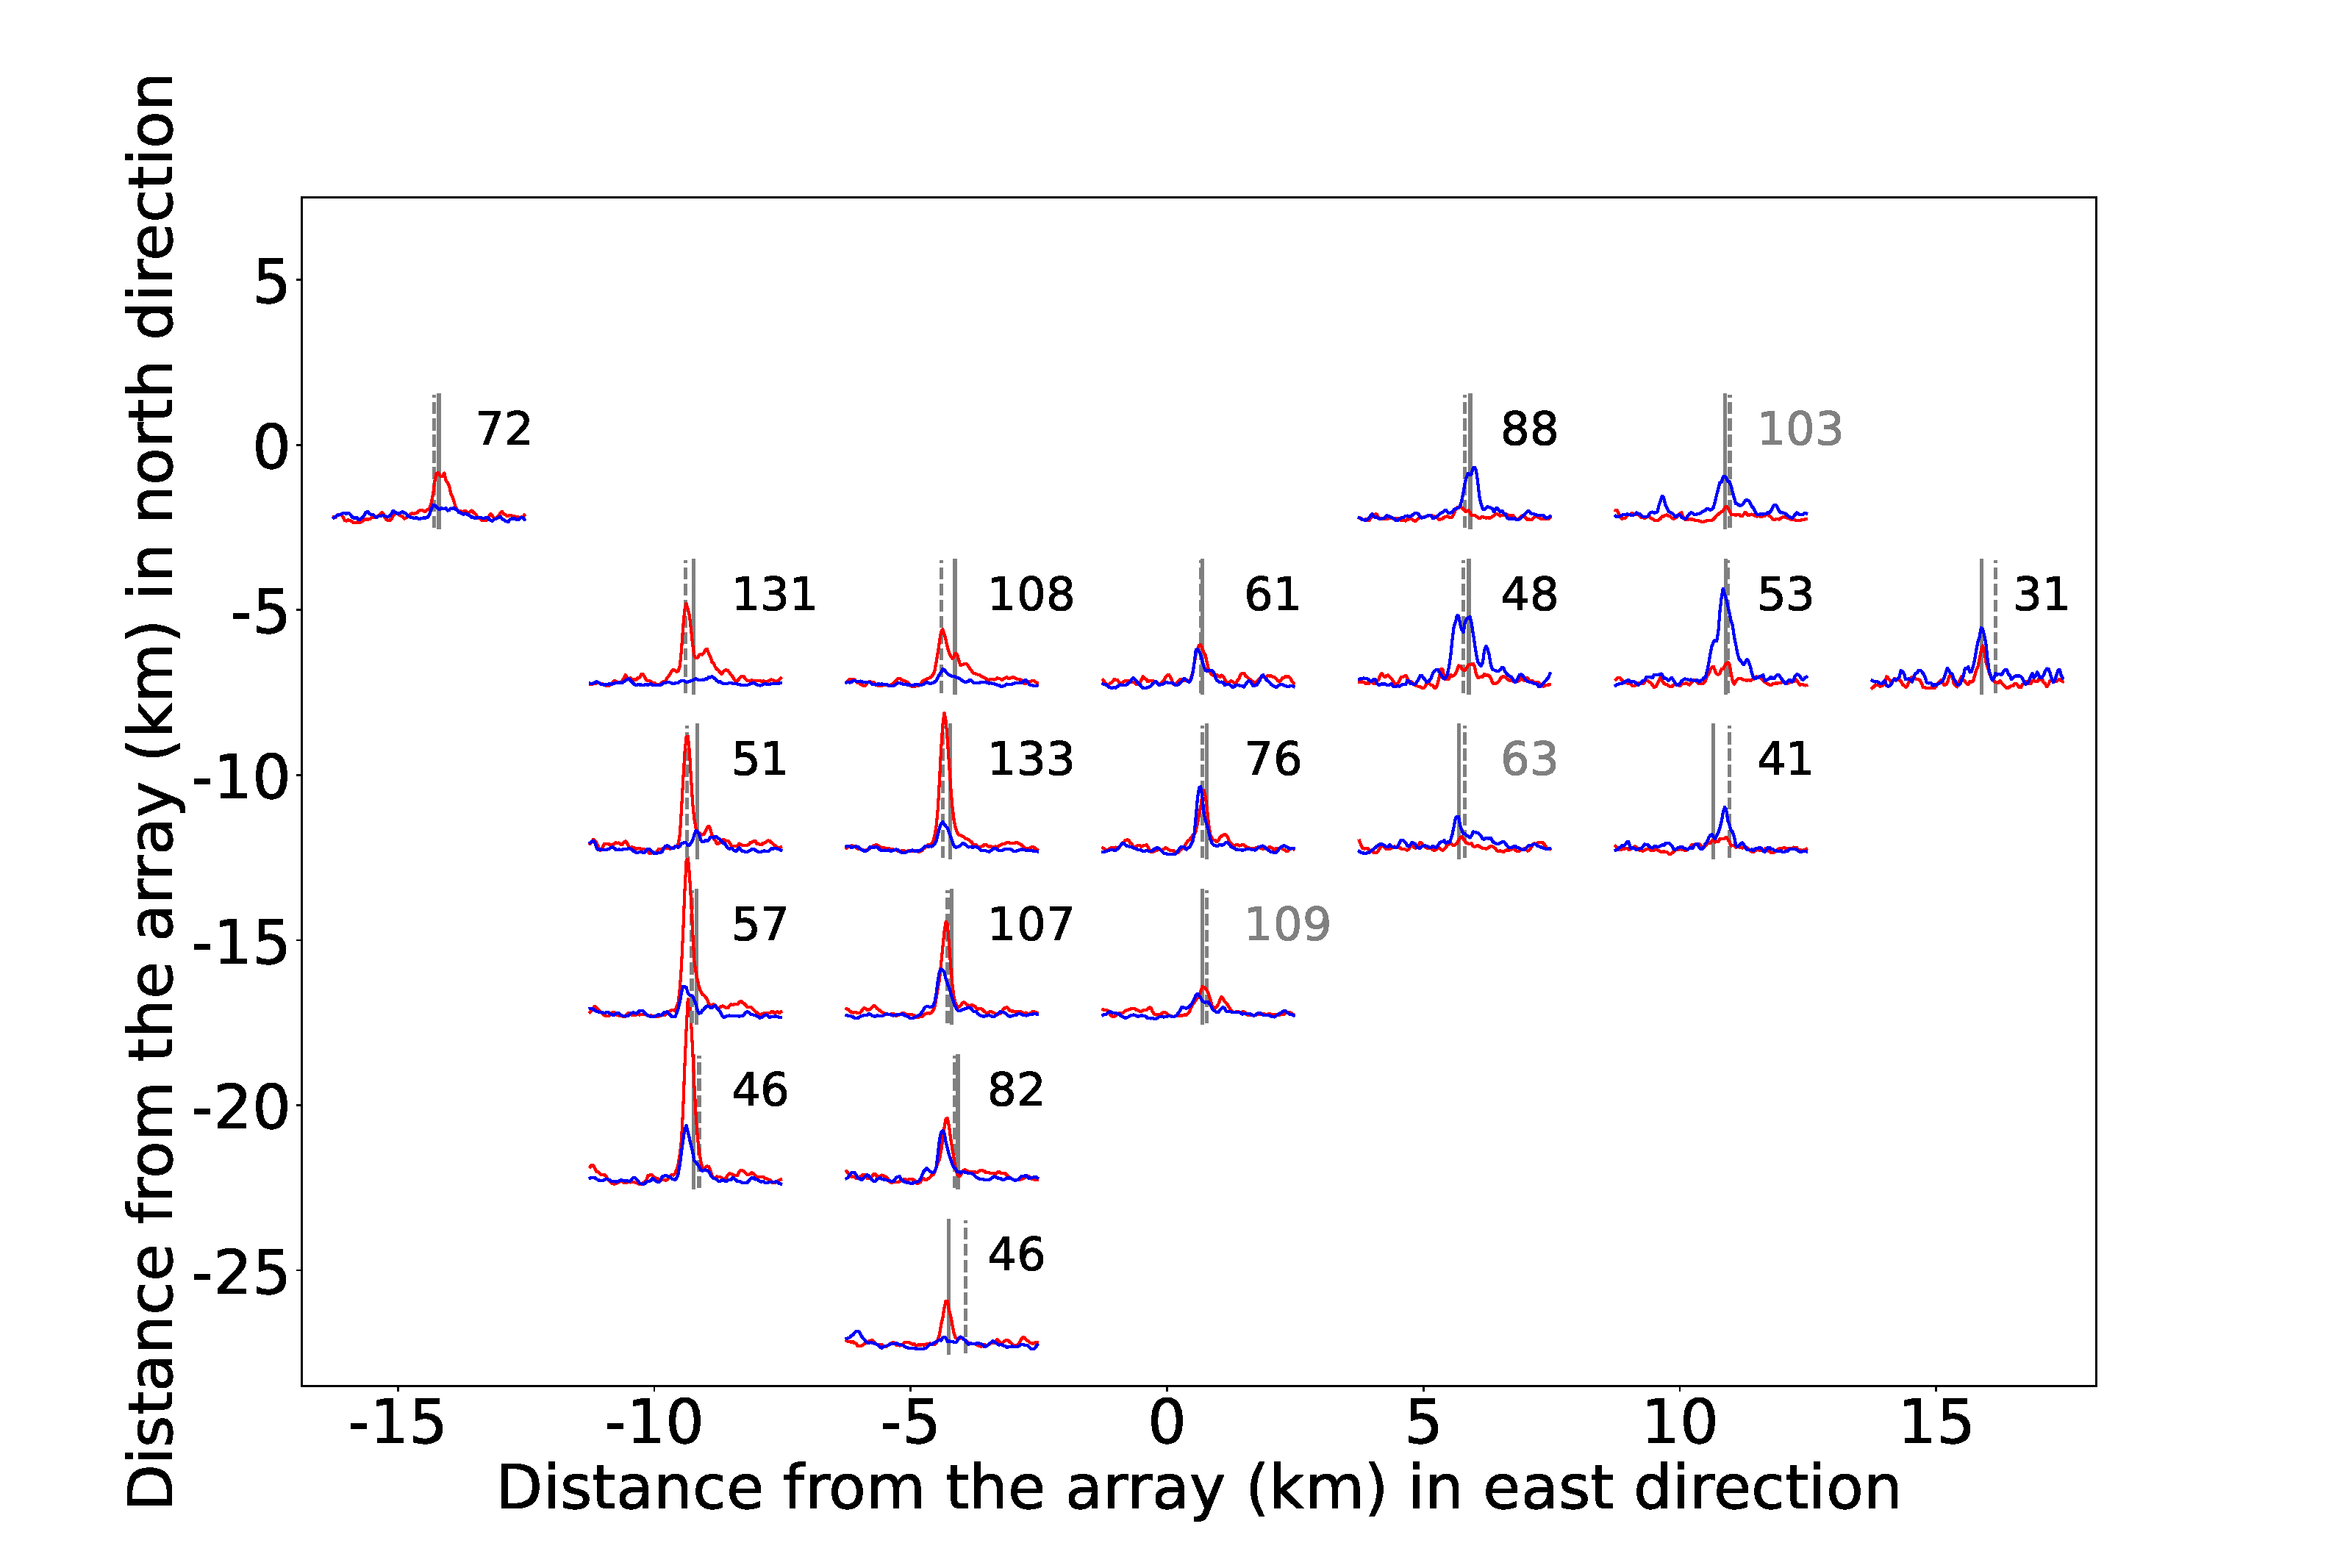
\includegraphics[width=\textwidth, trim={2.5cm 0.5cm 5cm 1.5cm},clip]{figures/TB_PWS_PWS_0.eps}
\caption{Stacks of the envelopes of the cross correlation signals for different positions of the tremor source relative to the Three Bumps array. See caption of Figure 4 for an explanation of this figure.}
\label{pngfiguresample}
\end{figure}

\begin{figure}
\noindent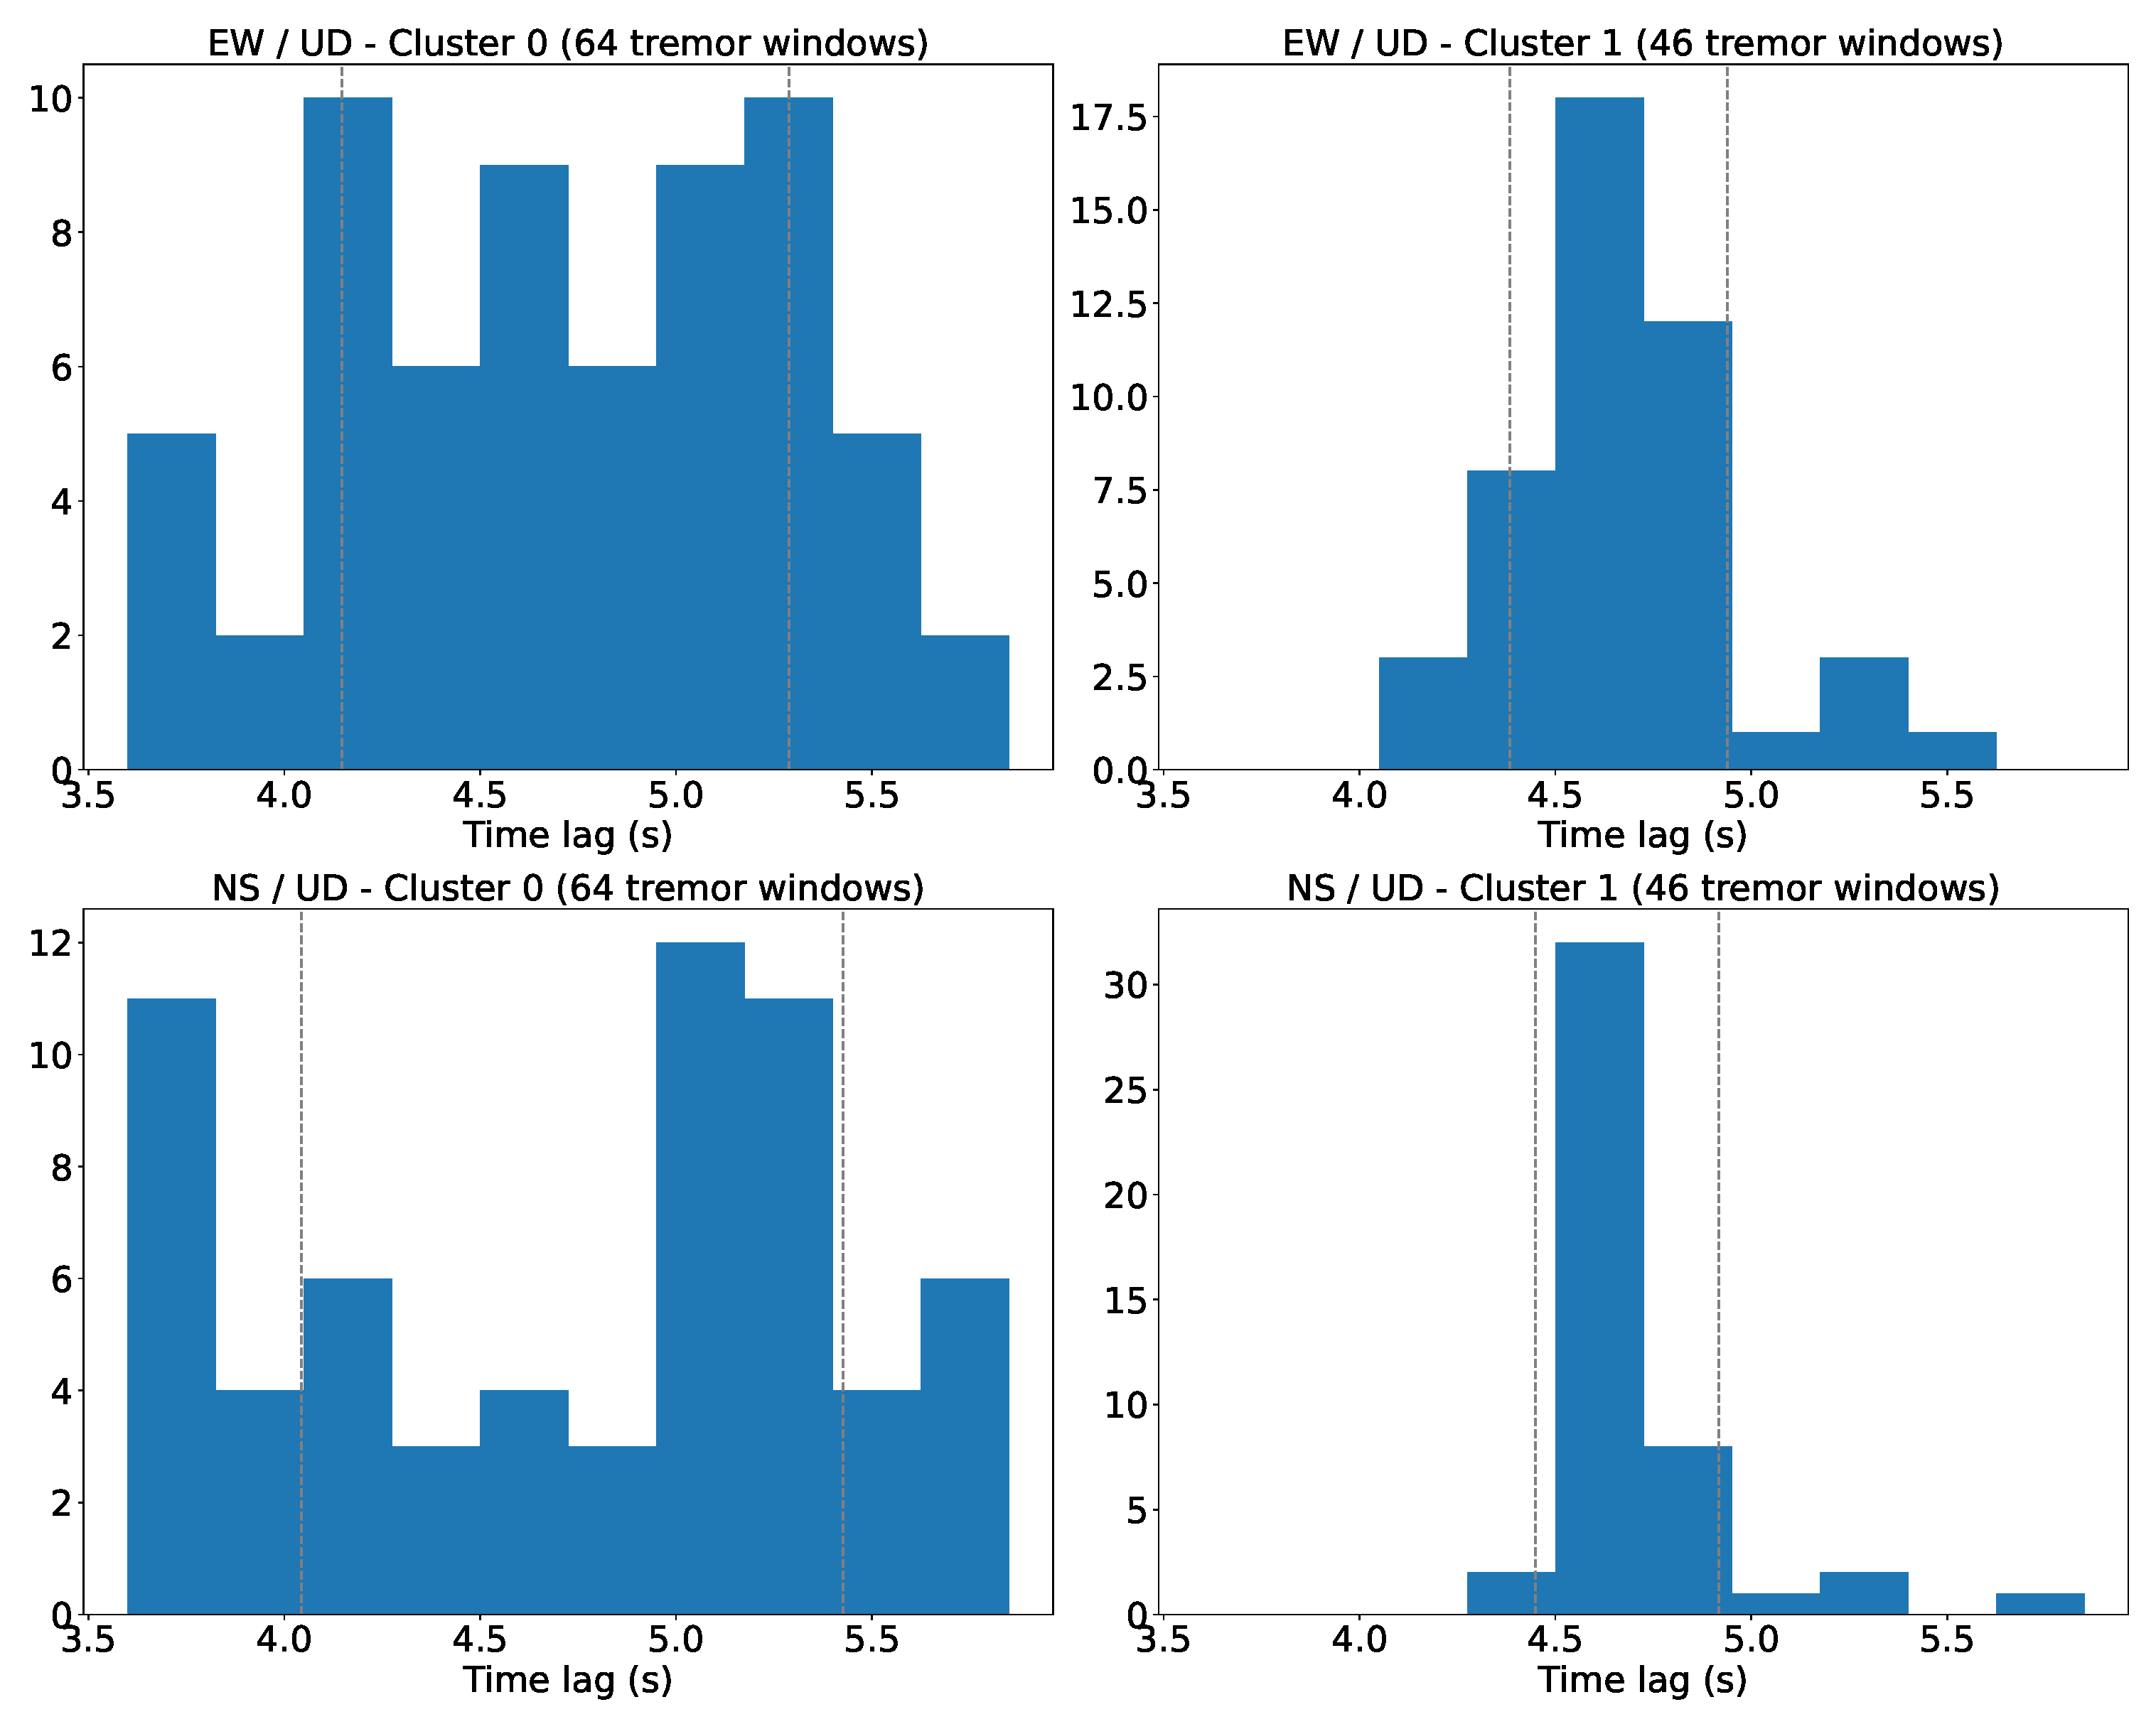
\includegraphics[width=\textwidth, trim={0cm 0cm 0cm 0cm},clip]{figures/BS_-05_-05_PWS_PWS_cluster_timelags.eps}
\caption{Distribution of the time lags between the time corresponding to the maximum absolute value for the cross-correlation function and the time corresponding to the maximum absolute value for the stacked cross-correlation for the time windows in cluster 0 (that is the time windows that do not fit well with the stack, left panel) and in cluster 1 (that is the time windows that fit well with the stack, right panel). Top panels are the cross-correlation of the EW component with the vertical component, and bottom panels are the cross-correlation of the NS component with the vertical component. The grey dashed lines correspond to the mean plus or minus the standard deviation. The array and the grid cell are the same as in Figures 1 and 2 of the main text.}
\label{pngfiguresample}
\end{figure}

\bibliography{bibliography}

\end{document}
